% begin module areas-intro
\begin{frame}
\frametitle{The Area Problem}
\begin{itemize}
\item  How can we find the area under $y = x^2$ between $x = 0$ and $x = 1$?
\item<handout:2-| 2->  We can approximate it using rectangles.
\item<handout:2-| 3->  Divide $[0,1]$ into three strips of width $\frac{1}{3}$, and draw rectangles in those strips, the heights of which are the same as the height of the function at the right end of that strip.
\item<handout:3-| 4->  Four strips gives a better approximation. \uncover<handout:0| 5->{Five is even better.}
\item<handout:6-| 11->  We could use the left endpoints to find the heights instead.
\end{itemize}
\ \uncover<handout:6-| 12>{\only<handout:-5| -12>{%
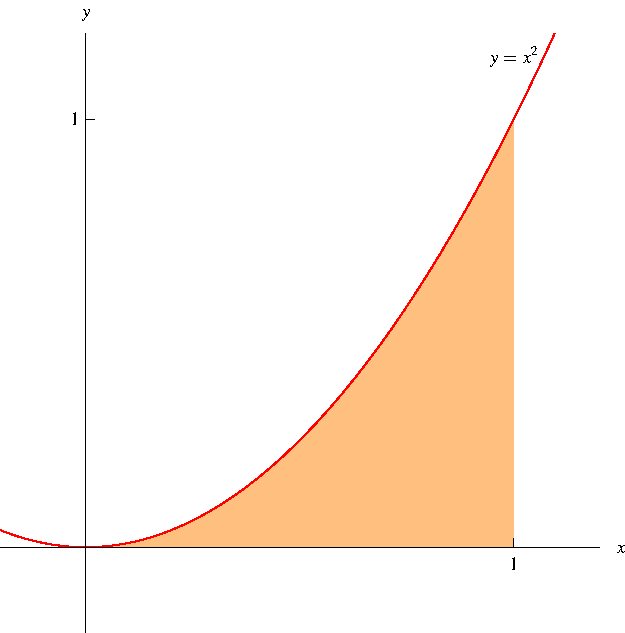
\includegraphics[height=4cm]{integration/pictures/05-01-xsquaredarea.pdf}%
}}%
\only<handout:6| 13>{%
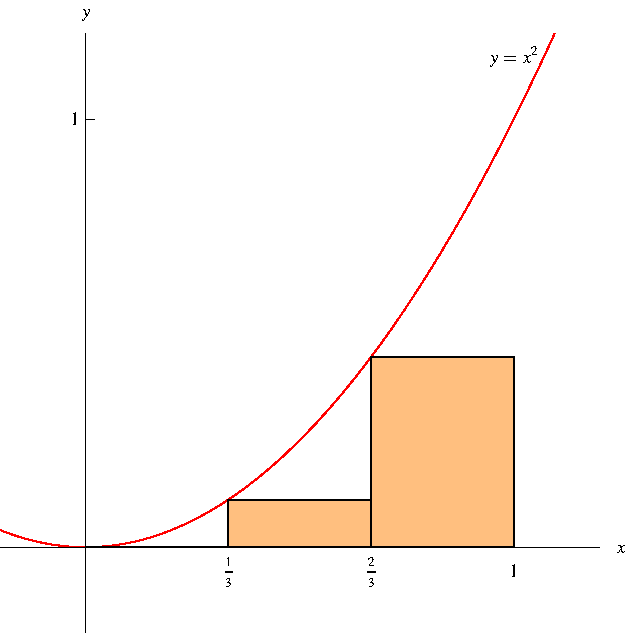
\includegraphics[height=4cm]{integration/pictures/05-01-lefta.pdf}%
}%
\only<handout:0| 14>{%
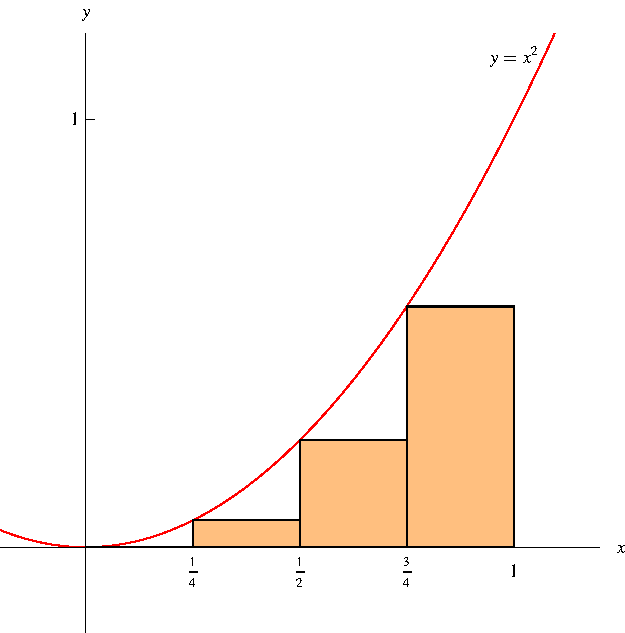
\includegraphics[height=4cm]{integration/pictures/05-01-leftb.pdf}%
}%
\only<handout:0| 15>{%
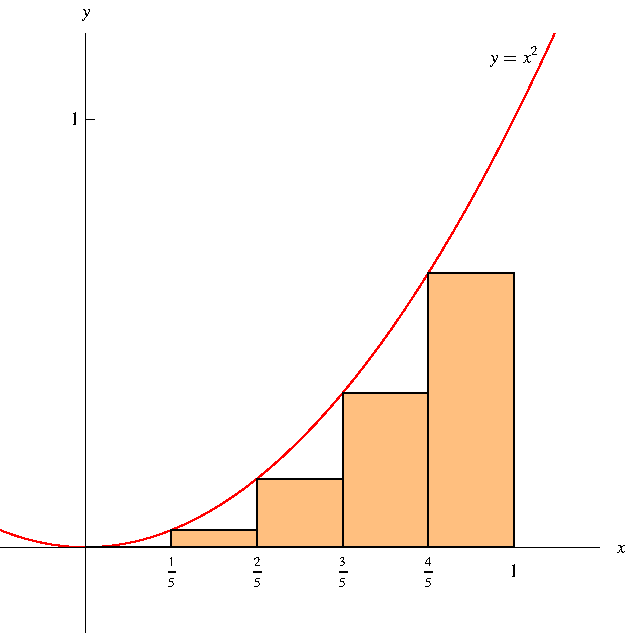
\includegraphics[height=4cm]{integration/pictures/05-01-leftc.pdf}%
}%
\only<handout:0| 16>{%
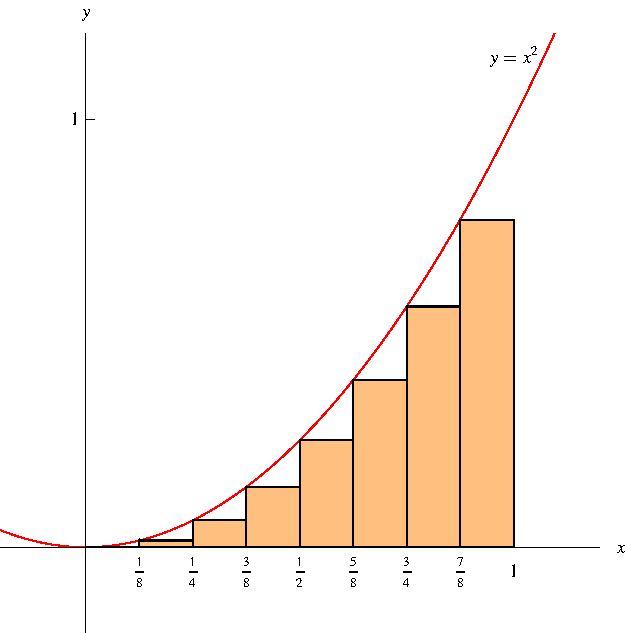
\includegraphics[height=4cm]{integration/pictures/05-01-leftd.pdf}%
}%
\only<handout:0| 17>{%
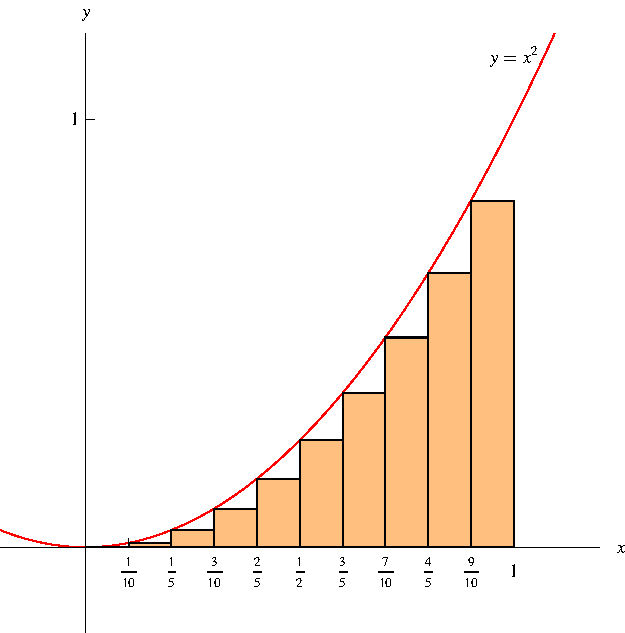
\includegraphics[height=4cm]{integration/pictures/05-01-lefte.pdf}%
}%
\only<handout:0| 18>{%
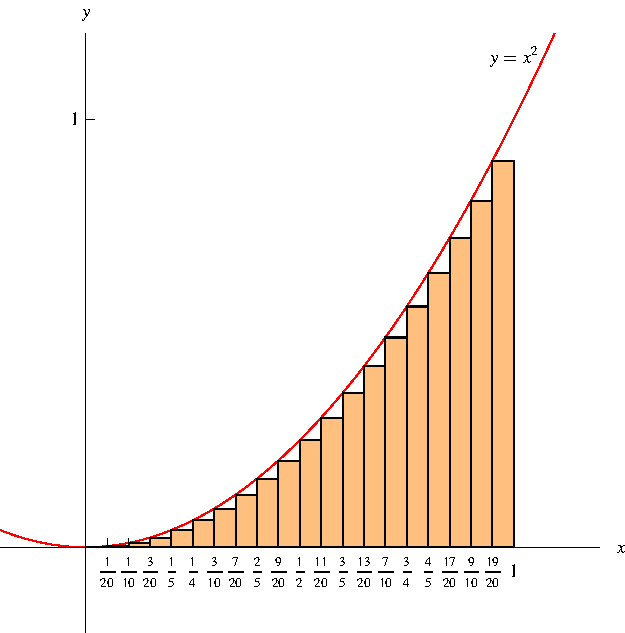
\includegraphics[height=4cm]{integration/pictures/05-01-leftf.pdf}%
}%
\only<handout:0| 19>{%
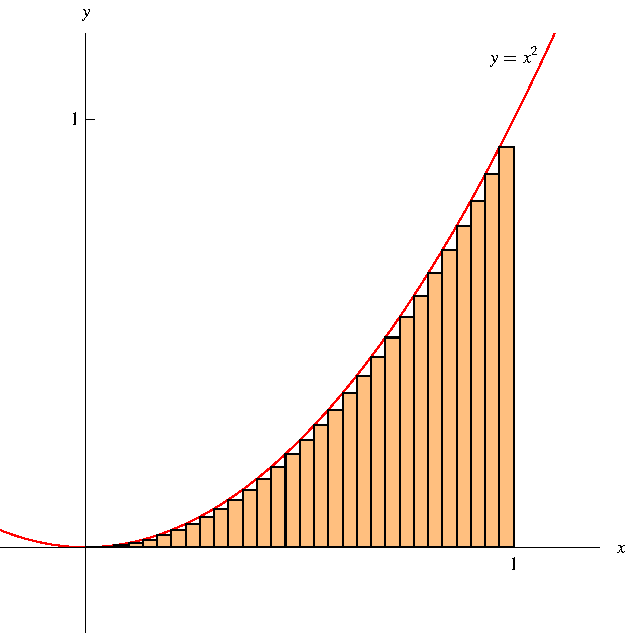
\includegraphics[height=4cm]{integration/pictures/05-01-leftg.pdf}%
}%
\only<handout:7| 20->{%
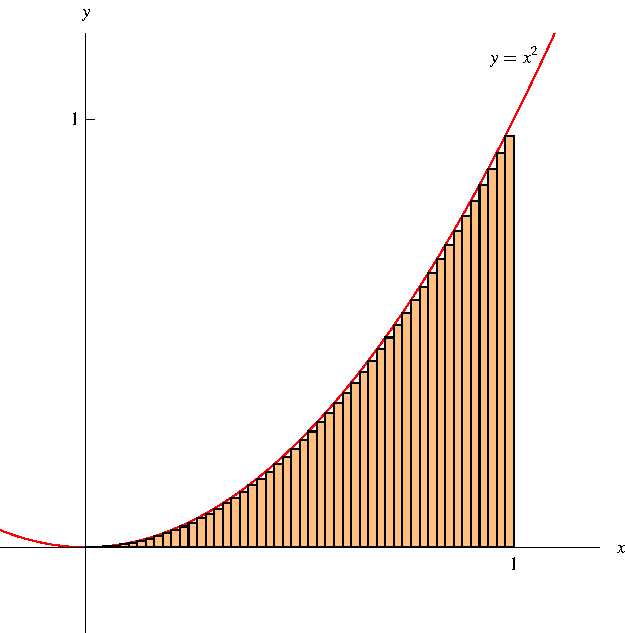
\includegraphics[height=4cm]{integration/pictures/05-01-lefth.pdf}%
}%
\ \only<handout:1| -2>{%
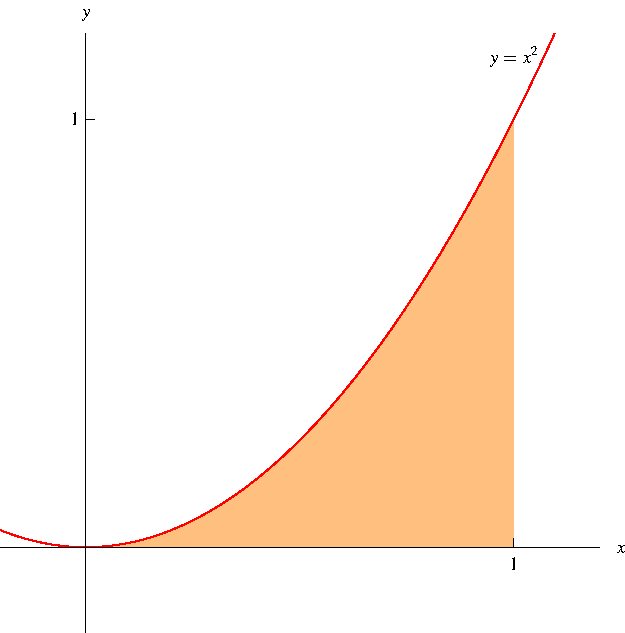
\includegraphics[height=4cm]{integration/pictures/05-01-xsquaredarea.pdf}%
}%
\only<handout:2| 3>{%
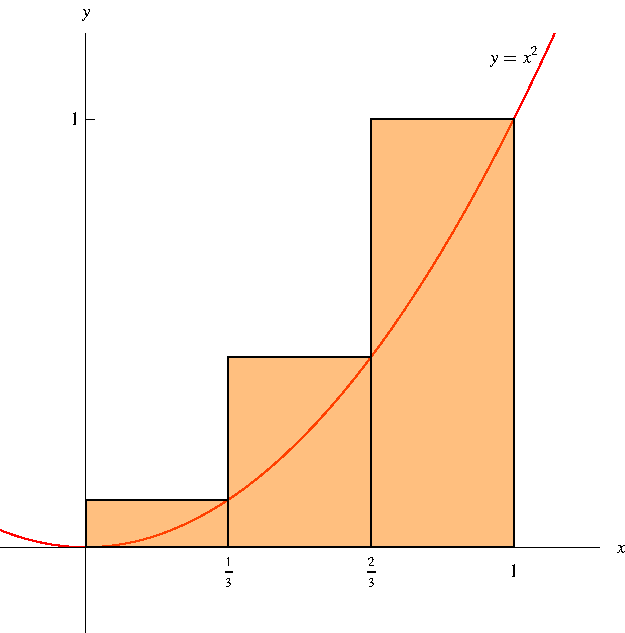
\includegraphics[height=4cm]{integration/pictures/05-01-righta.pdf}%
}%
\only<handout:3| 4>{%
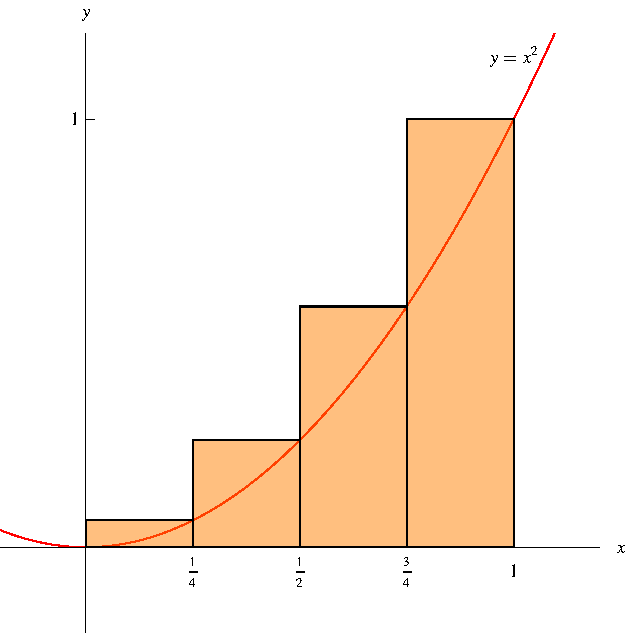
\includegraphics[height=4cm]{integration/pictures/05-01-rightb.pdf}%
}%
\only<handout:0| 5>{%
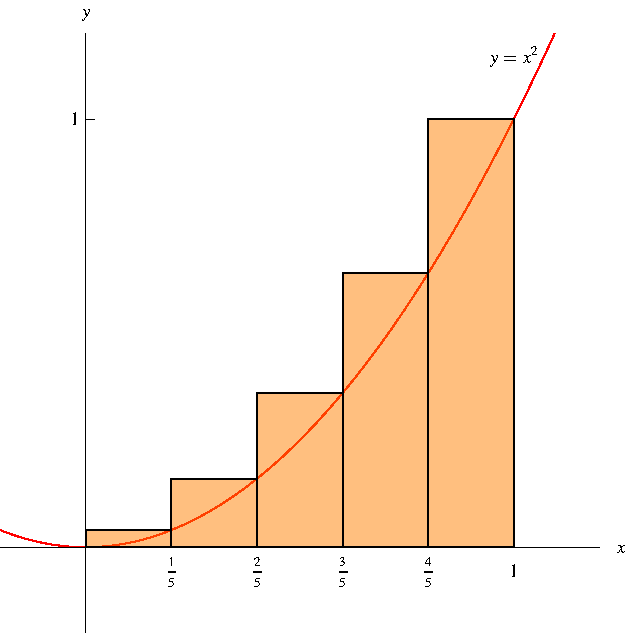
\includegraphics[height=4cm]{integration/pictures/05-01-rightc.pdf}%
}%
\only<handout:4| 6>{%
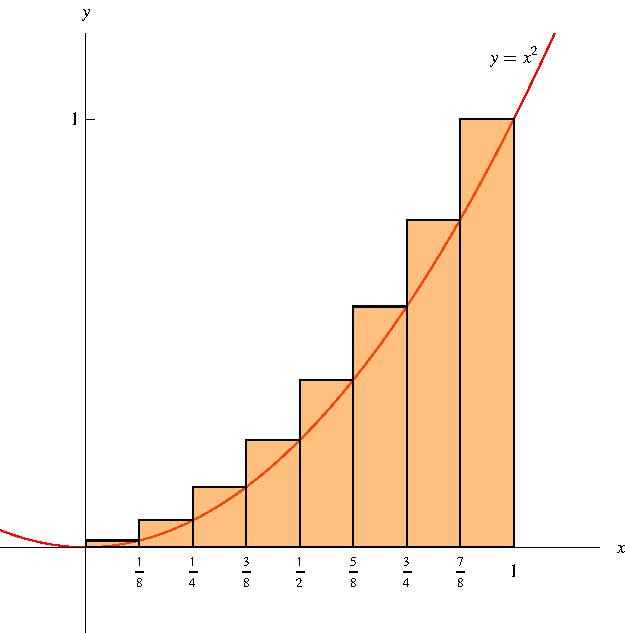
\includegraphics[height=4cm]{integration/pictures/05-01-rightd.pdf}%
}%
\only<handout:0| 7>{%
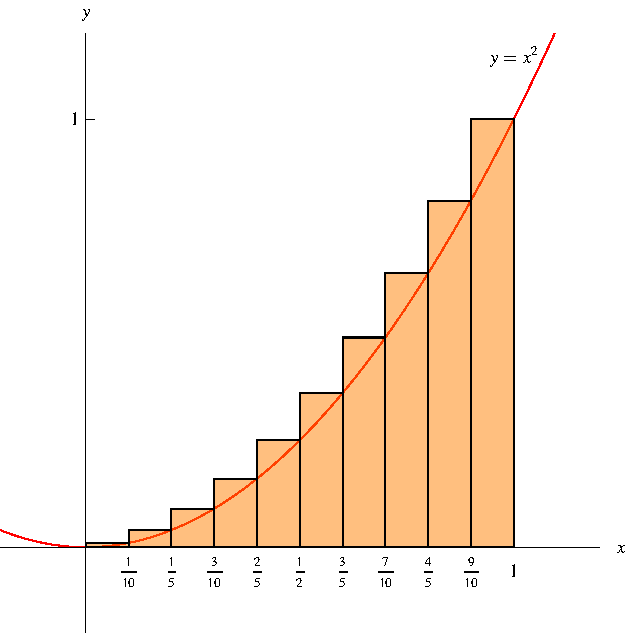
\includegraphics[height=4cm]{integration/pictures/05-01-righte.pdf}%
}%
\only<handout:0| 8>{%
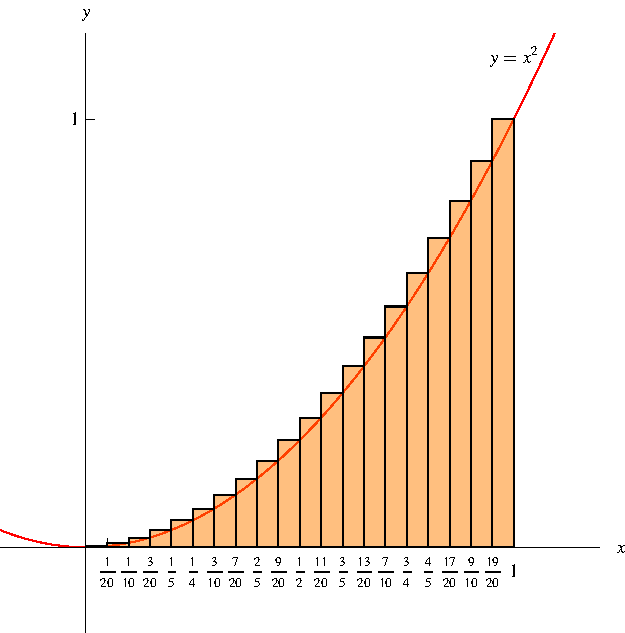
\includegraphics[height=4cm]{integration/pictures/05-01-rightf.pdf}%
}%
\only<handout:0| 9>{%
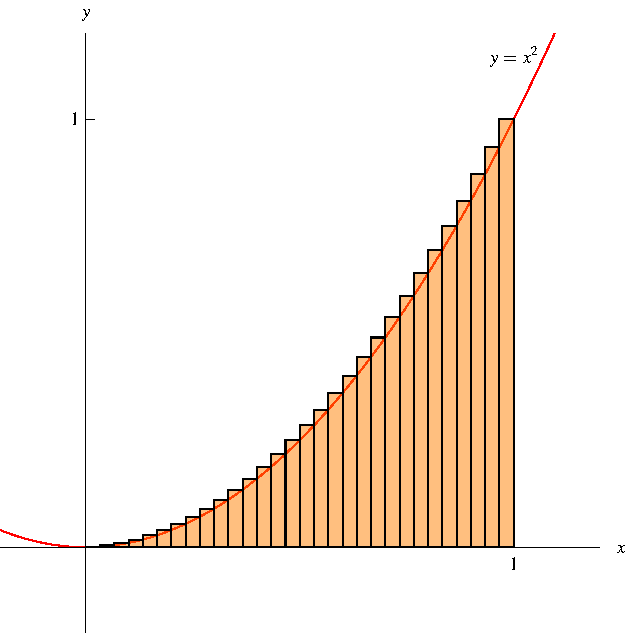
\includegraphics[height=4cm]{integration/pictures/05-01-rightg.pdf}%
}%
\only<handout:5-| 10->{%
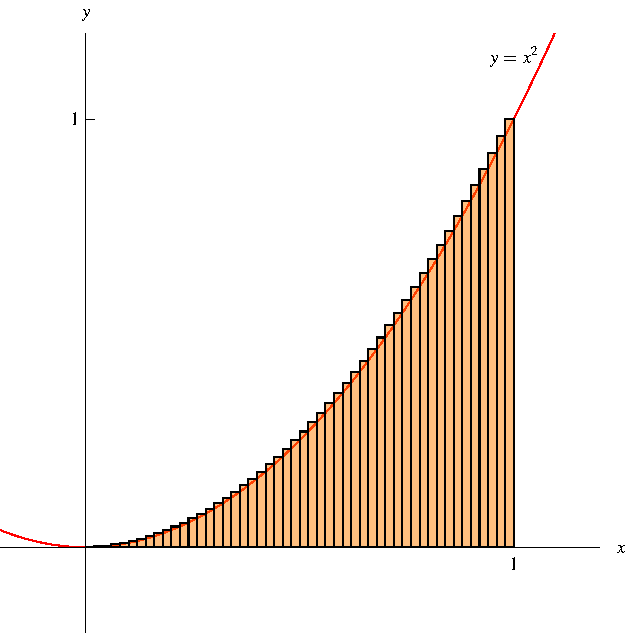
\includegraphics[height=4cm]{integration/pictures/05-01-righth.pdf}%
}%
\end{frame}
% end module areas-intro
